

\begin{figure}[h]

\centering


\begin{subfigure}[b]{0.49\textwidth}
\tikzsetnextfilename{APS2}

\centering
\resizebox{1\textwidth}{!}{
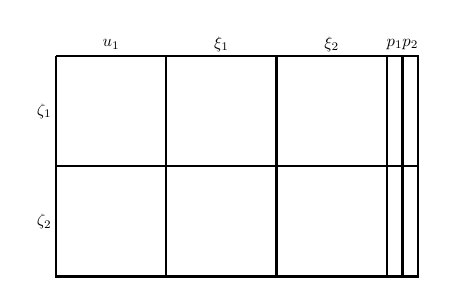
\begin{tikzpicture}[yscale=-1] 

\pgfmathsetmacro{\nt}{7};% time points
\pgfmathsetmacro{\nu}{1}; % controls
\pgfmathsetmacro{\nx}{2}; % states
\pgfmathsetmacro{\np}{2}; % parameters
\pgfmathsetmacro{\nc}{\nu + \nx}; % total continuous

%% control labels
\foreach \k in {1,...,\nu}{
	\pgfmathsetmacro{\x}{0.2*\nt*\k - 0.2/2*(\nt-1)};
	\node () at (\x,-0.05) {\scalebox{0.6}{$u_{\k}$}};
}

%% state labels
\foreach \k in {1,...,\nx}{
	\pgfmathsetmacro{\x}{0.2*\nt*\k + 0.2*\nu*\nt - 0.2/2*(\nt-1)};
	\node () at (\x,-0.05) {\scalebox{0.6}{$\xi_{\k}$}};
}

%% parameter labels
\foreach \k in {1,...,\np}{
	\pgfmathsetmacro{\x}{0.2*\k + 0.2*\nu*\nt + 0.2*\nx*\nt};
	\node () at (\x,-0.05) {\scalebox{0.6}{$p_{\k}$}};
}

%% defects
\foreach \k in {1,...,\nx}{
	\pgfmathsetmacro{\x}{0.2*\nt*\k - 0.2/2*(\nt-1)};
	\node () at (-0.05,\x) {\scalebox{0.6}{$\zeta_{\k}$}};
}


%% controls
\foreach \k in {1,...,\nu}{
	\foreach \j in {1,...,\nx}{
		\foreach \i in {1,...,\nt}{ 
        	\pgfmathsetmacro{\kk}{\k-1};
            \pgfmathsetmacro{\jj}{\j-1};
        	\pgfmathsetmacro{\x}{0.2*\i + 0.2*\kk*\nt};
            \pgfmathsetmacro{\y}{0.2*\i + 0.2*\jj*\nt};
        	\node () at (\x,\y) {\mysparsesymbol};
} 
    \pgfmathsetmacro{\kk}{\k-1};
    \pgfmathsetmacro{\jj}{\j-1};
    \pgfmathsetmacro{\x}{0.2*\kk*\nt + 0.1};
    \pgfmathsetmacro{\y}{0.2*\jj*\nt + 0.1};
	\draw[\mysparseboxcolor,thick](\x,\y) -- (\x+0.2*\nt,\y) -- (\x+0.2*\nt,\y+0.2*\nt) -- (\x,\y+0.2*\nt) -- (\x,\y);
} }

%% states
\foreach \k in {1,...,\nx}{
	\foreach \j in {1,...,\nx}{
		\foreach \i in {1,...,\nt}{ 
        	\pgfmathsetmacro{\kk}{\k-1};
            \pgfmathsetmacro{\jj}{\j-1};
        	\pgfmathsetmacro{\x}{0.2*\i + 0.2*\nu*\nt + 0.2*\kk*\nt};
            \pgfmathsetmacro{\y}{0.2*\i + 0.2*\jj*\nt};
        	\node () at (\x,\y) {\mysparsesymbol};
} 
    \pgfmathsetmacro{\kk}{\k-1};
    \pgfmathsetmacro{\jj}{\j-1};
    \pgfmathsetmacro{\x}{0.2*\kk*\nt + 0.2*\nu*\nt + 0.1};
    \pgfmathsetmacro{\y}{0.2*\jj*\nt + 0.1};
	\draw[\mysparseboxcolor,thick](\x,\y) -- (\x+0.2*\nt,\y) -- (\x+0.2*\nt,\y+0.2*\nt) -- (\x,\y+0.2*\nt) -- (\x,\y);
} }

%% states - full
\foreach \k in {1,...,\nx}{
		\foreach \i in {1,...,\nt}{
        	\foreach \p in {1,...,\nt}{
            
              \pgfmathsetmacro{\kk}{\k-1};
              \pgfmathsetmacro{\x}{0.2*\i + 0.2*\nu*\nt + 0.2*\kk*\nt};
              \pgfmathsetmacro{\y}{0.2*\p + 0.2*\kk*\nt};
            
        	\node () at (\x,\y) {\mysparsesymbol};
} } }

%% parameters
\foreach \k in {1,...,\np}{
	\foreach \j in {1,...,\nx}{
		\foreach \i in {1,...,\nt}{ 
        	\pgfmathsetmacro{\kk}{\k-1};
            \pgfmathsetmacro{\jj}{\j-1};
        	\node () at ( 0.2*\k + 0.2*\nx*\nt + 0.2*\nu*\nt, 0.2*\i + 0.2*\jj*\nt ) {\mysparsesymbol};
} 
    \pgfmathsetmacro{\kk}{\k-1};
    \pgfmathsetmacro{\jj}{\j-1};
    \pgfmathsetmacro{\x}{0.2*\kk + 0.2*\nx*\nt + 0.2*\nu*\nt + 0.1};
    \pgfmathsetmacro{\y}{0.2*\jj*\nt+ 0.1};
	\draw[\mysparseboxcolor,thick](\x,\y) -- (\x+0.2,\y) -- (\x+0.2,\y+0.2*\nt) -- (\x,\y+0.2*\nt) -- (\x,\y);

} }

%% states - full
\foreach \k in {1,...,\nx}{
		\foreach \i in {1,...,\nt}{
        	\foreach \p in {1,...,\nt}{
            
              \pgfmathsetmacro{\kk}{\k-1};
              \pgfmathsetmacro{\x}{0.2*\i + 0.2*\nu*\nt + 0.2*\kk*\nt};
              \pgfmathsetmacro{\y}{0.2*\p + 0.2*\kk*\nt};
            
        	\node () at (\x,\y) {\mytemp};
} } }

\end{tikzpicture}
}
\vspace{-5mm}
\caption{$\bm{D}$ terms.}
\end{subfigure}
%%%%%%%%%%%
\begin{subfigure}[b]{0.49\textwidth}
\tikzsetnextfilename{APS1}

\centering
\resizebox{1\textwidth}{!}{
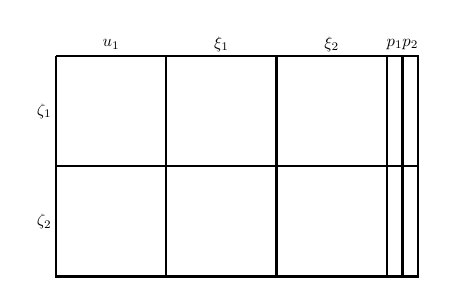
\begin{tikzpicture}[yscale=-1] 

\pgfmathsetmacro{\nt}{7};% time points
\pgfmathsetmacro{\nu}{1}; % controls
\pgfmathsetmacro{\nx}{2}; % states
\pgfmathsetmacro{\np}{2}; % parameters
\pgfmathsetmacro{\nc}{\nu + \nx}; % total continuous

%% control labels
\foreach \k in {1,...,\nu}{
	\pgfmathsetmacro{\x}{0.2*\nt*\k - 0.2/2*(\nt-1)};
	\node () at (\x,-0.05) {\scalebox{0.6}{$u_{\k}$}};
}

%% state labels
\foreach \k in {1,...,\nx}{
	\pgfmathsetmacro{\x}{0.2*\nt*\k + 0.2*\nu*\nt - 0.2/2*(\nt-1)};
	\node () at (\x,-0.05) {\scalebox{0.6}{$\xi_{\k}$}};
}

%% parameter labels
\foreach \k in {1,...,\np}{
	\pgfmathsetmacro{\x}{0.2*\k + 0.2*\nu*\nt + 0.2*\nx*\nt};
	\node () at (\x,-0.05) {\scalebox{0.6}{$p_{\k}$}};
}

%% defects
\foreach \k in {1,...,\nx}{
	\pgfmathsetmacro{\x}{0.2*\nt*\k - 0.2/2*(\nt-1)};
	\node () at (-0.05,\x) {\scalebox{0.6}{$\zeta_{\k}$}};
}


%% controls
\foreach \k in {1,...,\nu}{
	\foreach \j in {1,...,\nx}{
		\foreach \i in {1,...,\nt}{ 
        	\pgfmathsetmacro{\kk}{\k-1};
            \pgfmathsetmacro{\jj}{\j-1};
        	\pgfmathsetmacro{\x}{0.2*\i + 0.2*\kk*\nt};
            \pgfmathsetmacro{\y}{0.2*\i + 0.2*\jj*\nt};
        	\node () at (\x,\y) {\mysparsesymbol};
} 
    \pgfmathsetmacro{\kk}{\k-1};
    \pgfmathsetmacro{\jj}{\j-1};
    \pgfmathsetmacro{\x}{0.2*\kk*\nt + 0.1};
    \pgfmathsetmacro{\y}{0.2*\jj*\nt + 0.1};
	\draw[\mysparseboxcolor,thick](\x,\y) -- (\x+0.2*\nt,\y) -- (\x+0.2*\nt,\y+0.2*\nt) -- (\x,\y+0.2*\nt) -- (\x,\y);
} }

%% states
\foreach \k in {1,...,\nx}{
	\foreach \j in {1,...,\nx}{
		\foreach \i in {1,...,\nt}{ 
        	\pgfmathsetmacro{\kk}{\k-1};
            \pgfmathsetmacro{\jj}{\j-1};
        	\pgfmathsetmacro{\x}{0.2*\i + 0.2*\nu*\nt + 0.2*\kk*\nt};
            \pgfmathsetmacro{\y}{0.2*\i + 0.2*\jj*\nt};
        	\node () at (\x,\y) {\mysparsesymbol};
} 
    \pgfmathsetmacro{\kk}{\k-1};
    \pgfmathsetmacro{\jj}{\j-1};
    \pgfmathsetmacro{\x}{0.2*\kk*\nt + 0.2*\nu*\nt + 0.1};
    \pgfmathsetmacro{\y}{0.2*\jj*\nt + 0.1};
	\draw[\mysparseboxcolor,thick](\x,\y) -- (\x+0.2*\nt,\y) -- (\x+0.2*\nt,\y+0.2*\nt) -- (\x,\y+0.2*\nt) -- (\x,\y);
} }

%% states - full
\foreach \k in {1,...,\nx}{
		\foreach \i in {1,...,\nt}{
        	\foreach \p in {1,...,\nt}{
            
              \pgfmathsetmacro{\kk}{\k-1};
              \pgfmathsetmacro{\x}{0.2*\i + 0.2*\nu*\nt + 0.2*\kk*\nt};
              \pgfmathsetmacro{\y}{0.2*\p + 0.2*\kk*\nt};
            
        	\node () at (\x,\y) {\mysparsesymbol};
} } }

%% parameters
\foreach \k in {1,...,\np}{
	\foreach \j in {1,...,\nx}{
		\foreach \i in {1,...,\nt}{ 
        	\pgfmathsetmacro{\kk}{\k-1};
            \pgfmathsetmacro{\jj}{\j-1};
        	\node () at ( 0.2*\k + 0.2*\nx*\nt + 0.2*\nu*\nt, 0.2*\i + 0.2*\jj*\nt ) {\mysparsesymbol};
} 
    \pgfmathsetmacro{\kk}{\k-1};
    \pgfmathsetmacro{\jj}{\j-1};
    \pgfmathsetmacro{\x}{0.2*\kk + 0.2*\nx*\nt + 0.2*\nu*\nt + 0.1};
    \pgfmathsetmacro{\y}{0.2*\jj*\nt+ 0.1};
	\draw[\mysparseboxcolor,thick](\x,\y) -- (\x+0.2,\y) -- (\x+0.2,\y+0.2*\nt) -- (\x,\y+0.2*\nt) -- (\x,\y);

} }

%% states
\foreach \k in {1,...,\nx}{
	\foreach \j in {1,...,\nx}{
		\foreach \i in {1,...,\nt}{ 
        	\pgfmathsetmacro{\kk}{\k-1};
            \pgfmathsetmacro{\jj}{\j-1};
        	\pgfmathsetmacro{\x}{0.2*\i + 0.2*\nu*\nt + 0.2*\kk*\nt};
            \pgfmathsetmacro{\y}{0.2*\i + 0.2*\jj*\nt};
        	\node () at (\x,\y) {\mytemp};
} } }

\end{tikzpicture}
}
\vspace{-5mm}
\caption{$\bm{A}$ terms.}
\end{subfigure}


\begin{subfigure}[b]{0.49\textwidth}
\input{../ch5/sparsity/APS3}
\vspace{-5mm}
\caption{$\bm{B}$ terms.}
\end{subfigure}
%%%%%%%%%%%
\begin{subfigure}[b]{0.49\textwidth}
\tikzsetnextfilename{APS4}

\centering
\resizebox{1\textwidth}{!}{
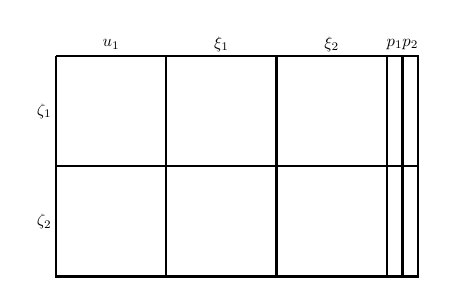
\begin{tikzpicture}[yscale=-1] 

\pgfmathsetmacro{\nt}{7};% time points
\pgfmathsetmacro{\nu}{1}; % controls
\pgfmathsetmacro{\nx}{2}; % states
\pgfmathsetmacro{\np}{2}; % parameters
\pgfmathsetmacro{\nc}{\nu + \nx}; % total continuous

%% control labels
\foreach \k in {1,...,\nu}{
	\pgfmathsetmacro{\x}{0.2*\nt*\k - 0.2/2*(\nt-1)};
	\node () at (\x,-0.05) {\scalebox{0.6}{$u_{\k}$}};
}

%% state labels
\foreach \k in {1,...,\nx}{
	\pgfmathsetmacro{\x}{0.2*\nt*\k + 0.2*\nu*\nt - 0.2/2*(\nt-1)};
	\node () at (\x,-0.05) {\scalebox{0.6}{$\xi_{\k}$}};
}

%% parameter labels
\foreach \k in {1,...,\np}{
	\pgfmathsetmacro{\x}{0.2*\k + 0.2*\nu*\nt + 0.2*\nx*\nt};
	\node () at (\x,-0.05) {\scalebox{0.6}{$p_{\k}$}};
}

%% defects
\foreach \k in {1,...,\nx}{
	\pgfmathsetmacro{\x}{0.2*\nt*\k - 0.2/2*(\nt-1)};
	\node () at (-0.05,\x) {\scalebox{0.6}{$\zeta_{\k}$}};
}


%% controls
\foreach \k in {1,...,\nu}{
	\foreach \j in {1,...,\nx}{
		\foreach \i in {1,...,\nt}{ 
        	\pgfmathsetmacro{\kk}{\k-1};
            \pgfmathsetmacro{\jj}{\j-1};
        	\pgfmathsetmacro{\x}{0.2*\i + 0.2*\kk*\nt};
            \pgfmathsetmacro{\y}{0.2*\i + 0.2*\jj*\nt};
        	\node () at (\x,\y) {\mysparsesymbol};
} 
    \pgfmathsetmacro{\kk}{\k-1};
    \pgfmathsetmacro{\jj}{\j-1};
    \pgfmathsetmacro{\x}{0.2*\kk*\nt + 0.1};
    \pgfmathsetmacro{\y}{0.2*\jj*\nt + 0.1};
	\draw[\mysparseboxcolor,thick](\x,\y) -- (\x+0.2*\nt,\y) -- (\x+0.2*\nt,\y+0.2*\nt) -- (\x,\y+0.2*\nt) -- (\x,\y);
} }

%% states
\foreach \k in {1,...,\nx}{
	\foreach \j in {1,...,\nx}{
		\foreach \i in {1,...,\nt}{ 
        	\pgfmathsetmacro{\kk}{\k-1};
            \pgfmathsetmacro{\jj}{\j-1};
        	\pgfmathsetmacro{\x}{0.2*\i + 0.2*\nu*\nt + 0.2*\kk*\nt};
            \pgfmathsetmacro{\y}{0.2*\i + 0.2*\jj*\nt};
        	\node () at (\x,\y) {\mysparsesymbol};
} 
    \pgfmathsetmacro{\kk}{\k-1};
    \pgfmathsetmacro{\jj}{\j-1};
    \pgfmathsetmacro{\x}{0.2*\kk*\nt + 0.2*\nu*\nt + 0.1};
    \pgfmathsetmacro{\y}{0.2*\jj*\nt + 0.1};
	\draw[\mysparseboxcolor,thick](\x,\y) -- (\x+0.2*\nt,\y) -- (\x+0.2*\nt,\y+0.2*\nt) -- (\x,\y+0.2*\nt) -- (\x,\y);
} }

%% states - full
\foreach \k in {1,...,\nx}{
		\foreach \i in {1,...,\nt}{
        	\foreach \p in {1,...,\nt}{
            
              \pgfmathsetmacro{\kk}{\k-1};
              \pgfmathsetmacro{\x}{0.2*\i + 0.2*\nu*\nt + 0.2*\kk*\nt};
              \pgfmathsetmacro{\y}{0.2*\p + 0.2*\kk*\nt};
            
        	\node () at (\x,\y) {\mysparsesymbol};
} } }

%% parameters
\foreach \k in {1,...,\np}{
	\foreach \j in {1,...,\nx}{
		\foreach \i in {1,...,\nt}{ 
        	\pgfmathsetmacro{\kk}{\k-1};
            \pgfmathsetmacro{\jj}{\j-1};
        	\node () at ( 0.2*\k + 0.2*\nx*\nt + 0.2*\nu*\nt, 0.2*\i + 0.2*\jj*\nt ) {\mysparsesymbol};
} 
    \pgfmathsetmacro{\kk}{\k-1};
    \pgfmathsetmacro{\jj}{\j-1};
    \pgfmathsetmacro{\x}{0.2*\kk + 0.2*\nx*\nt + 0.2*\nu*\nt + 0.1};
    \pgfmathsetmacro{\y}{0.2*\jj*\nt+ 0.1};
	\draw[\mysparseboxcolor,thick](\x,\y) -- (\x+0.2,\y) -- (\x+0.2,\y+0.2*\nt) -- (\x,\y+0.2*\nt) -- (\x,\y);

} }

%% parameters
\foreach \k in {1,...,\np}{
	\foreach \j in {1,...,\nx}{
		\foreach \i in {1,...,\nt}{ 
        	\pgfmathsetmacro{\kk}{\k-1};
            \pgfmathsetmacro{\jj}{\j-1};
        	\node () at ( 0.2*\k + 0.2*\nx*\nt + 0.2*\nu*\nt, 0.2*\i + 0.2*\jj*\nt ) {\mytemp};
} } }

\end{tikzpicture}
}
\vspace{-5mm}
\caption{$\bm{G}$ terms.}
\end{subfigure}


\caption{Sparsity pattern of $\bm{\mathcal{A}}_e^1$ matrix for the defect constraints using a pseudospectral method.\label{fig:figsparsityAPS}}
\end{figure}